\documentclass{article}
\usepackage{fancyhdr}
\usepackage{ctex}
\usepackage{listings}
\usepackage{graphicx}
\usepackage[a4paper, body={18cm,22cm}]{geometry}
\usepackage{amsmath,amssymb,amstext,wasysym,enumerate,graphicx}
\usepackage{float,abstract,booktabs,indentfirst,amsmath}
\usepackage{array}
\usepackage{booktabs}
\usepackage{multirow}
\usepackage{url}
\usepackage{diagbox}
\renewcommand\arraystretch{1.4}
\usepackage{indentfirst}
\setlength{\parindent}{2em}
\usepackage{enumitem}
\setmonofont{DejaVu Sans Mono}
\usepackage{listings}
\usepackage{xcolor}
\usepackage{makecell}
\setCJKmonofont{黑体}
\usepackage{tikz}
\usepackage{tabularx}
\usetikzlibrary{positioning, arrows.meta}
\lstset{
    % language = C,
    xleftmargin = 3em,xrightmargin = 3em, aboveskip = 1em,
	backgroundcolor = \color{white}, % 背景色
	basicstyle = \small\ttfamily, % 基本样式 + 小号字体
	rulesepcolor= \color{gray}, % 代码块边框颜色
	breaklines = true, % 代码过长则换行
	numbers = left, % 行号在左侧显示
	numberstyle = \small, % 行号字体
    numbersep = -14pt, 
    keywordstyle=\color{purple}\bfseries, % 关键字颜色
    commentstyle =\color{red!50!green!50!blue!60}, % 注释颜色
    stringstyle = \color{red}, % 字符串颜色
    morekeywords={ASSERT, int64_t, uint32_t},
	frame = shadowbox, % 用(带影子效果)方框框住代码块
	showspaces = false, % 不显示空格
	columns = fixed, % 字间距固定
} 
\lstset{
    sensitive=true,
    moreemph={ASSERT, NULL}, emphstyle=\color{red}\bfseries,
    moreemph=[2]{int64_t, uint32_t, tid_t, uint8_t, int16_t, uint16_t, int32_t, size_t}, emphstyle=[2]\color{purple}\bfseries,
    }
%--------------------页眉--------------------%
\pagestyle{fancy}
\fancyhead[L]{}
\fancyhead[R]{}
\fancyhead[C]{华东师范大学软件工程学院实验报告}
\fancyfoot[C]{-\thepage-}
\renewcommand{\headrulewidth}{1.5pt}
%--------------------标题--------------------%
\begin{document}
\begin{center}
  \LARGE{{\textbf{\heiti 华东师范大学软件工程学院实验报告}}}
  \begin{table}[H]
    \centering
    \begin{tabular}{p{2cm}p{4cm}<{\centering}p{1cm}p{2cm}p{4cm}<{\centering}}
      实验课程:    & 计算机网络 & \quad & 年\qquad 级: & 2022级      \\ \cline{2-2} \cline{5-5}
      实验编号:    & Lab 04     & \quad & 实验名称:    & ARP
      \\ \cline{2-2} \cline{5-5}
      姓\qquad 名: & 李鹏达     & \quad & 学\qquad 号: & 10225101460 \\ \cline{2-2} \cline{5-5}
    \end{tabular}
  \end{table}
\end{center}
\rule{\textwidth}{1pt}
%--------------------正文--------------------%
\section{实验目的}
\begin{enumerate}[noitemsep, label={{\arabic*})}]
  \item 通过Wireshark获取ARP消息
  \item 掌握ARP数据包结构
  \item 掌握ARP数据包各字段的含义
  \item 了解ARP协议适用领域
\end{enumerate}
\section{实验内容与实验步骤}
\subsection{实验内容}


\subsubsection{捕获数据}

启动 \texttt{Wireshark},在菜单栏的捕获\(\to \)选项中进行设置,选择已连接的以太网,设置捕获过滤器为\texttt{arp},捕获\texttt{arp}数据包。

然后在命令行中使用\texttt{ipconfig -all}命令获取本机的\texttt{IP}地址和\texttt{MAC}地址。

在 \texttt{Wireshark} 的过滤器中输入\texttt{eth.addr==<yourMAC>
}(其中 \texttt{<yourMAC>}为本机的 \texttt{MAC}地址)。

在管理员模式下,使用 \texttt{arp -d} 命令清除本机的 \texttt{ARP} 缓存。

打开 \texttt{Wireshark},停止捕获。
\subsubsection{回答问题}

\begin{enumerate}[noitemsep]
  \item 画出你的计算机和本地路由间ARP的请求和应答数据包,标记出请求和应答,为每个数据包 给出发送者和接受者的MAC和IP地址。
  \item 什么样的操作码是用来表示一个请求?应答呢?
  \item 一个请求的ARP的报头有多大?应答呢?
  \item 对未知目标的MAC地址的请求是什么值?
  \item 什么以太网类型值说明ARP是更高一层的协议?
  \item ARP应答是广播吗?

\end{enumerate}


\subsubsection{问题讨论}

We encourage you to explore ARP on your own once you have completed this lab. One suggestion is to look at other ARP packets that may have been recorded in your trace; we only examined an ARP request by your computer and the ARP reply from the default gateway.

To see if there is other ARP activity, make sure to clear any Ethernet address filter that is set. Other ARP packets may exhibit any of the following kinds of behavior for you to explore:

\begin{enumerate}[noitemsep]
  \item ARP requests broadcast by other computers. The other computers on the local network are also using ARP. Since requests are broadcast, your computer will receive their requests.
  \item ARP replies sent by your computer. If another computer happens to ARP for the IP address of your computer, then your computer will send an ARP reply to tell it the answer.
  \item Gratuitous ARPs in which your computer sends a request or reply about itself. This is helpful when a computer or link comes up to make sure that no-one else is using the same IP address. Gratuitous ARPs have the same sender and target IP address, and they have an Info field in Wireshark that identified them as gratuitous.
  \item Other ARP requests sent by your computer and the corresponding ARP reply. Your computer may need to ARP for other hosts besides the default gateway after you flush its ARP cache.
\end{enumerate}



\subsection{实验步骤}

\begin{enumerate}[noitemsep, label={{\arabic*})}]
  \item 启动\texttt{Wireshark},在菜单栏的捕获\(\to \)选项中进行设置,选择已连接的以太网,设置捕获过滤器为\texttt{arp},将混杂模式设为关闭,然后开始捕获。
  \item 在命令行中使用\texttt{ipconfig -all}命令获取本机的\texttt{IP}地址和\texttt{MAC}地址。
        \begin{lstlisting}
    PS> ipconfig -all
  \end{lstlisting}
  \item 回到\texttt{Wireshark},设置捕获过滤器为 \texttt{eth.addr==<yourMAC>
        }
  \item 在管理员模式下,使用 \texttt{arp -d} 命令清除本机的 \texttt{ARP} 缓存。
        \begin{lstlisting}
    PS> arp -d
  \end{lstlisting}
  \item 打开 \texttt{Wireshark},停止捕获。
  \item 分析捕获到的\texttt{ARP}数据包,并回答相关问题。
  \item 对捕获到的\texttt{ARP}数据包进行数据分析,并回答相关问题。
  \item 问题讨论
\end{enumerate}

\section{实验环境}


\begin{itemize}[noitemsep]
  \item 操作系统:\texttt{Windows 11 家庭中文版 23H2 22631.2715}
  \item 网络适配器:\texttt{Killer(R) Wi-Fi 6 AX1650i 160MHz Wireless Network Adapter(201NGW)}
  \item \texttt{Wireshark}:\texttt{Version 4.2.0 (v4.2.0-0-g54eedfc63953)}
  \item \texttt{wget}:\texttt{GNU Wget 1.21.4 built on mingw32}
\end{itemize}


\section{实验结果与分析}

\subsection{捕获数据}

首先,打开\texttt{Wireshark},在菜单栏的捕获\(\to \)选项中进行设置,选择已连接的以太网,设置捕获过滤器为\texttt{arp},将混杂模式设为关闭,然后开始捕获。

\begin{figure}[H]
  \centering
  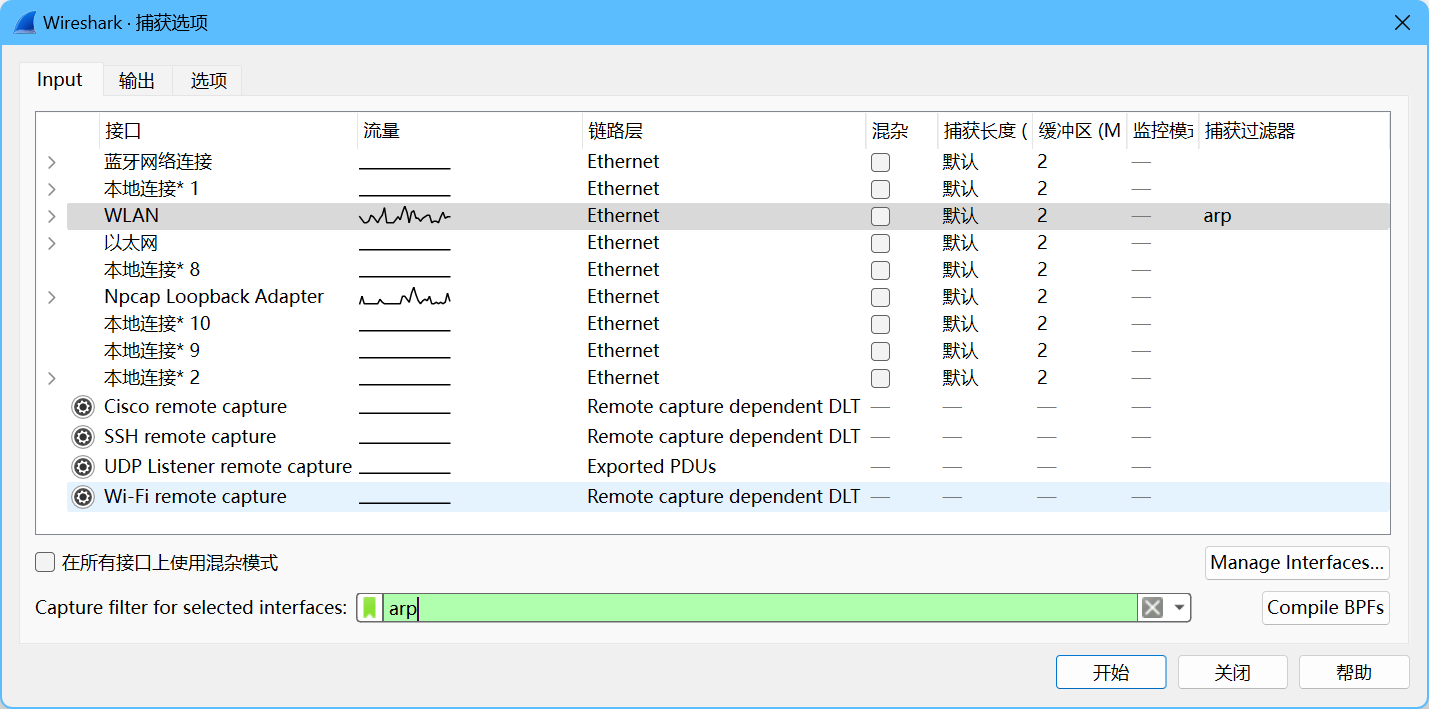
\includegraphics[width=0.8\textwidth]{img/1.png}
  \caption{设置捕获选项}
  \label{fig:1}
\end{figure}

然后在命令行中使用\texttt{ipconfig -all}命令获取本机的\texttt{IP}地址和\texttt{MAC}地址。

\begin{figure}[H]
  \centering
  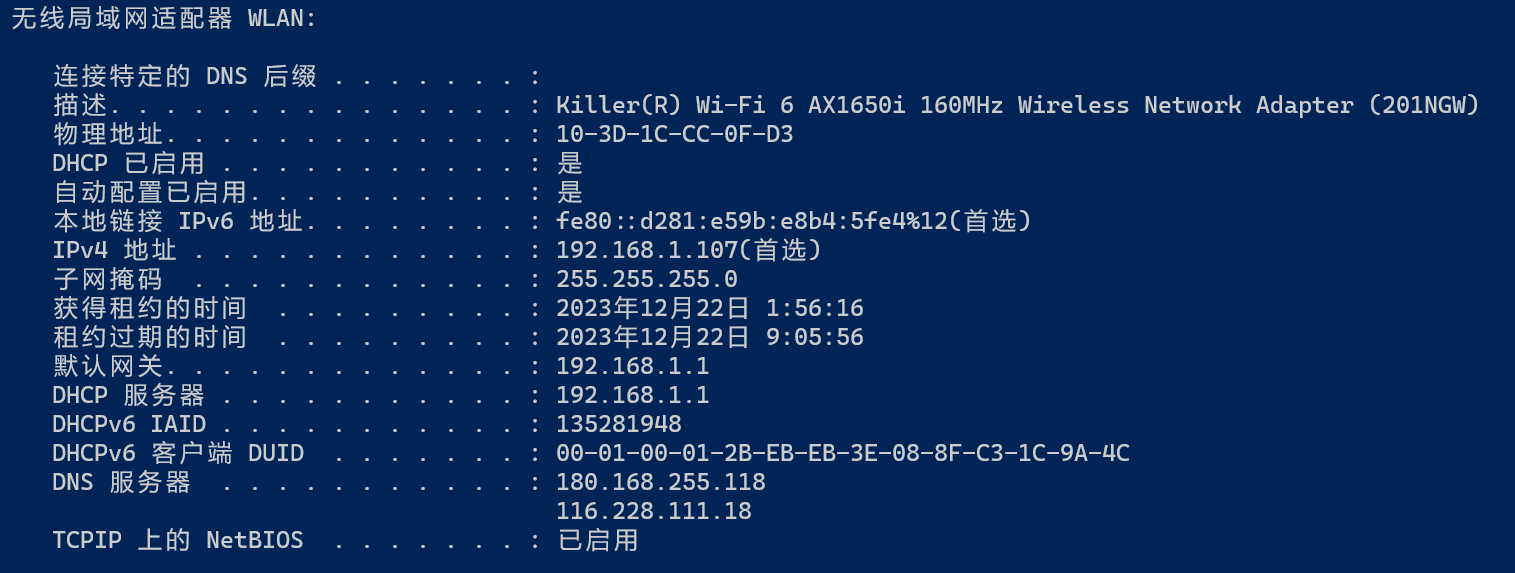
\includegraphics[width=0.8\textwidth]{img/2.png}
  \caption{获取本机\texttt{IP}地址和\texttt{MAC}地址}
  \label{fig:2}
\end{figure}

可以看到,本机的 \texttt{IP} 地址为 \texttt{192.168.1.107}, \texttt{MAC} 地址为 \texttt{10-3D-1C-CC-0F-D3}。

回到\texttt{Wireshark},设置捕获过滤器为 \texttt{eth.addr==10-3D-1C-CC-0F-D3}。

\begin{figure}[H]
  \centering
  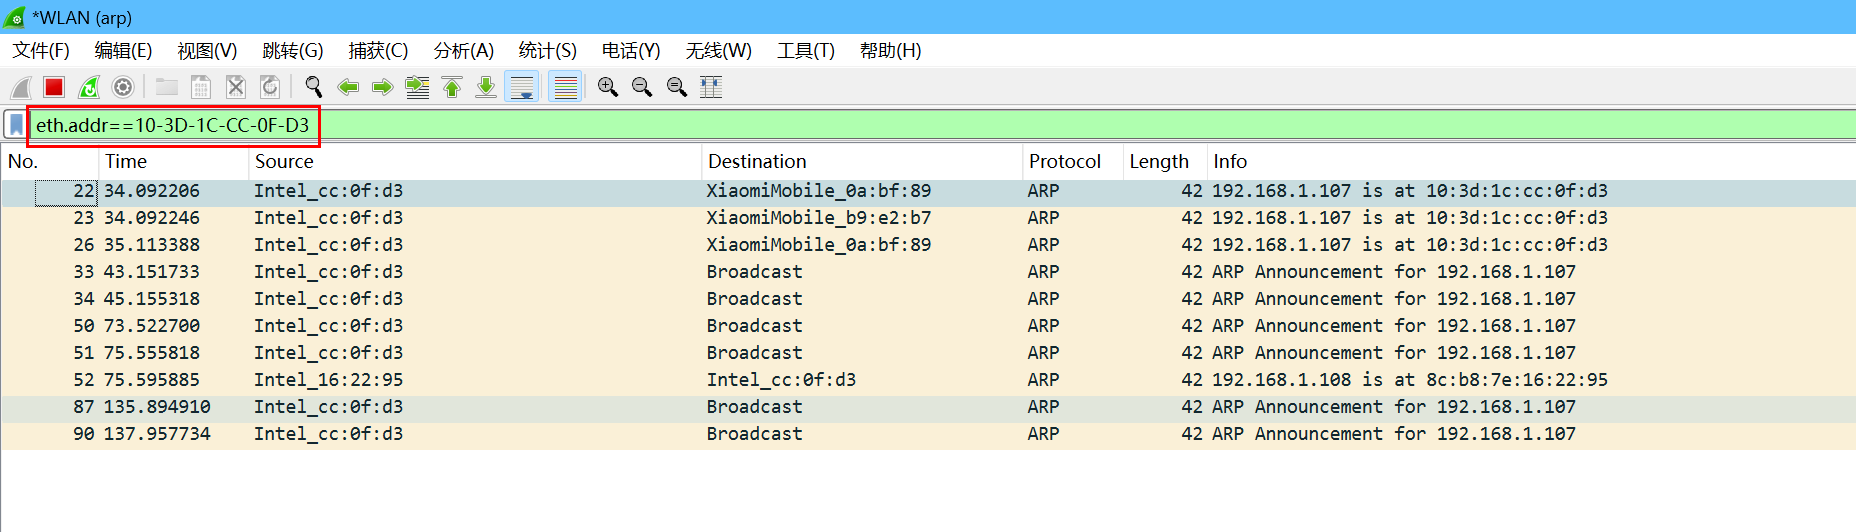
\includegraphics[width=0.8\textwidth]{img/3.png}
  \caption{设置捕获过滤器}
  \label{fig:3}
\end{figure}

接下来,在管理员模式下,在终端中使用 \texttt{arp -d} 命令清除本机的 \texttt{ARP} 缓存。

\begin{figure}[H]
  \centering
  
\includegraphics[width=0.3\textwidth]{img/4.png}
  \caption{清除本机\texttt{ARP}缓存}
  \label{fig:4}
\end{figure}

打开 \texttt{Wireshark},停止捕获。捕获结果如下图所示:

\begin{figure}[H]
  \centering
  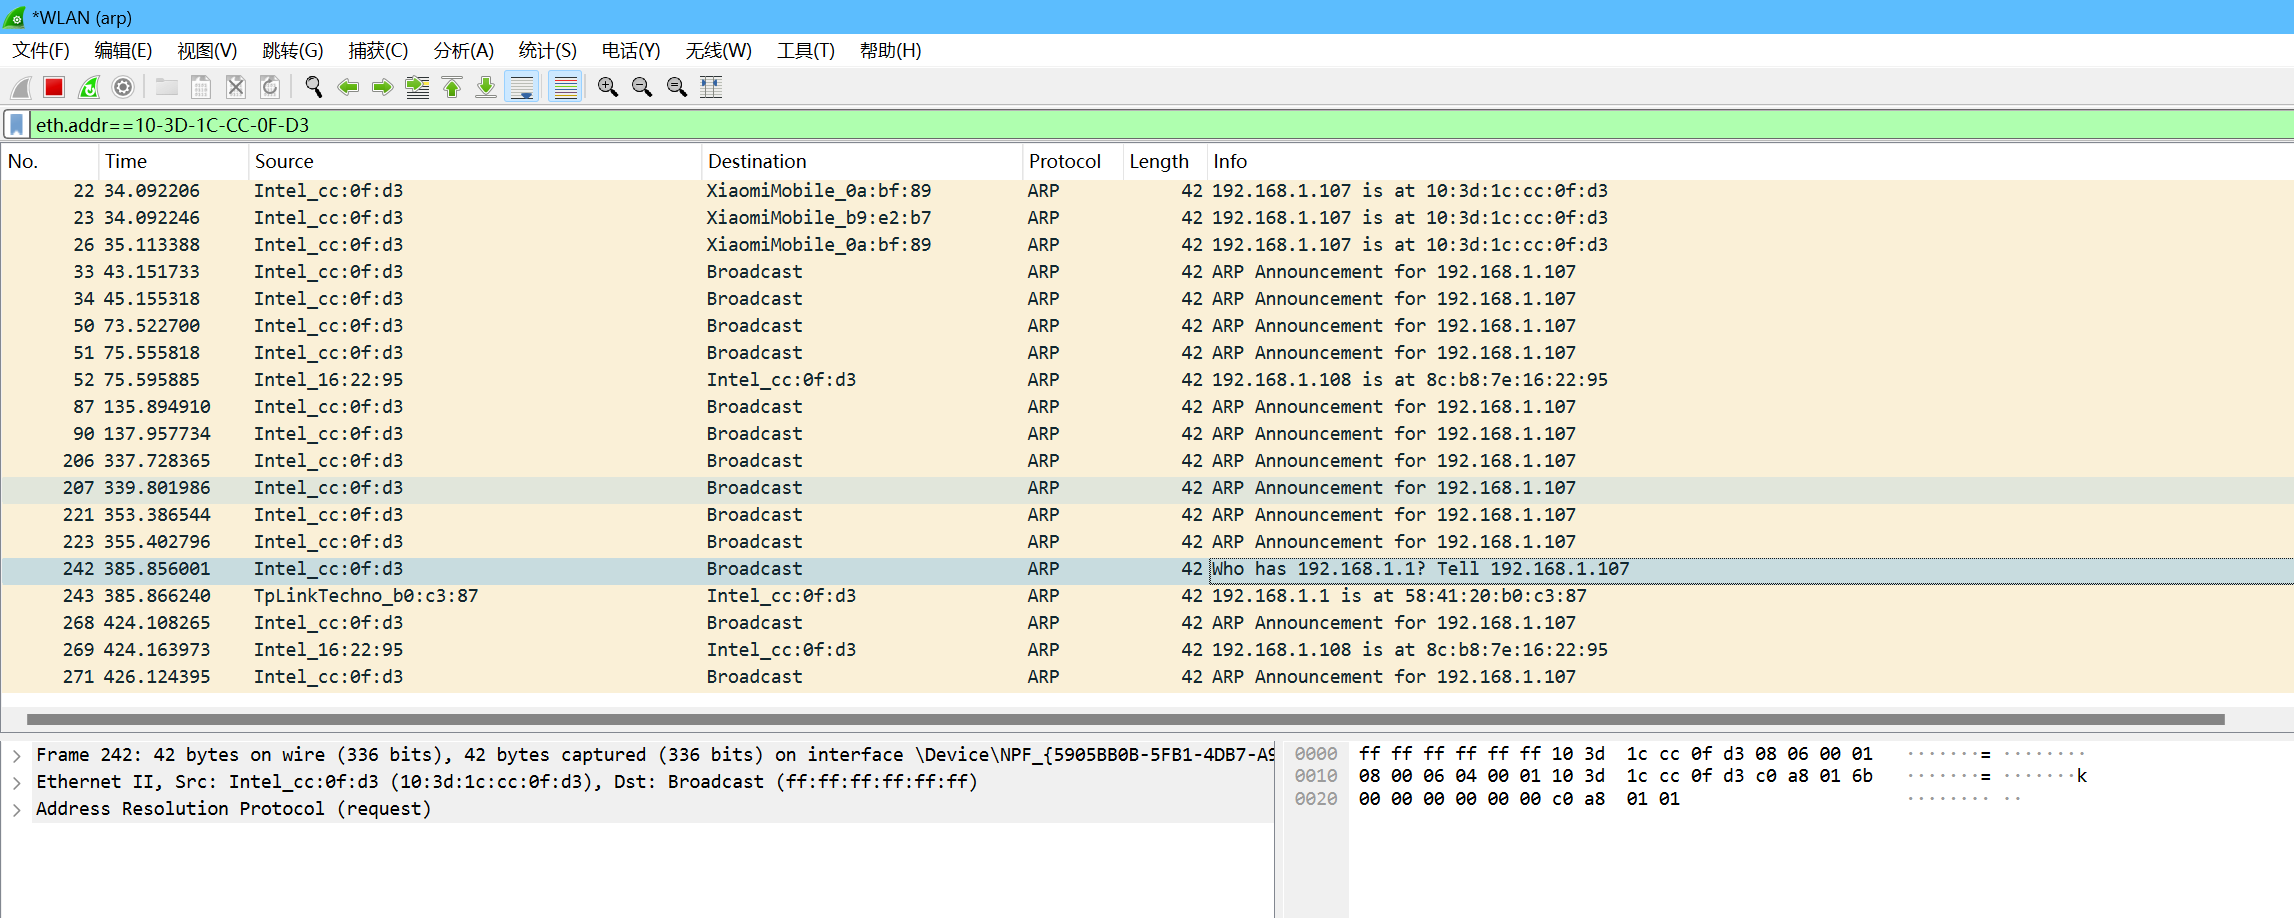
\includegraphics[width=0.8\textwidth]{img/5.png}
  \caption{捕获结果}
  \label{fig:5}
\end{figure}

\subsection{回答问题}

\begin{enumerate}[noitemsep]
  \item 画出你的计算机和本地路由间ARP的请求和应答数据包,标记出请求和应答,为每个数据包 给出发送者和接受者的MAC和IP地址。

        选择 \texttt{ARP} 请求数据包,如下图所示:

        \begin{figure}[H]
          \centering
          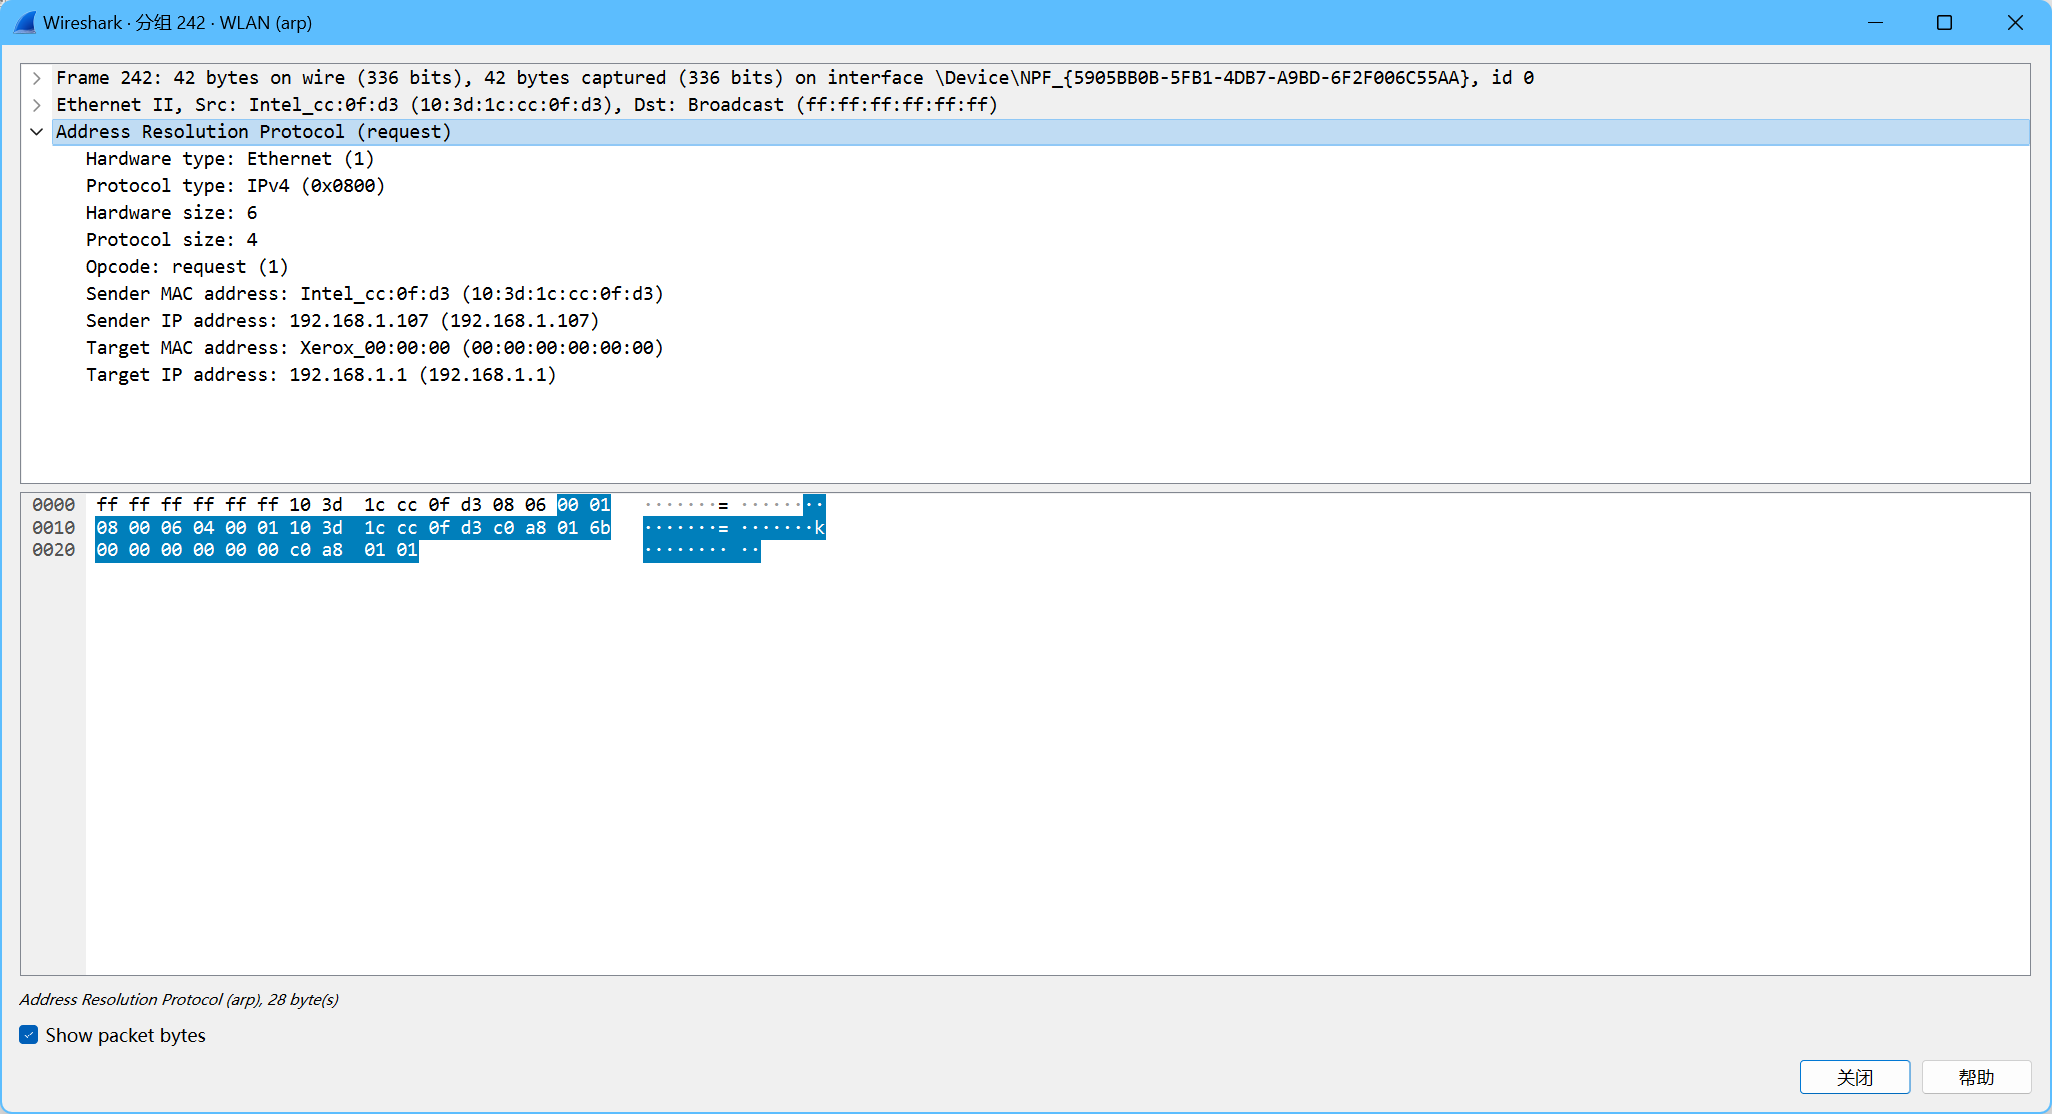
\includegraphics[width=0.8\textwidth]{img/6.png}
          \caption{选择\texttt{ARP}请求数据包}
          \label{fig:6}
        \end{figure}

        可以看到,它包括了一个长度为 28 字节的 \texttt{ARP} 报头,其中包括了以下字段:

        \begin{itemize}[noitemsep]
          \item Hardware type: Ethernet (1),长度为 2 字节
          \item Protocol type: \texttt{IPv4}(0x0800),长度为 2 字节
          \item Hardware size: 6,长度为 1 字节
          \item Protocol size: 4,长度为 1 字节
          \item Opcode: request (1),长度为 2 字节
          \item Sender MAC address: \texttt{10:3d:1c:cc:0f:d3},长度为 6 字节
          \item Sender IP address: \texttt{192.168.1.107},长度为 4 字节
          \item Target MAC address: \texttt{00:00:00:00:00:00},长度为 6 字节
          \item Target IP address: \texttt{192.168.1.1},长度为 4 字节
        \end{itemize}

        画出 \texttt{ARP} 请求数据包,如下图所示:

        % 10 列的表格
        \begin{table}[H]
          \centering
          \begin{tabularx}{0.78\textwidth}{|*{10}{X|}}
            \hline
            \multicolumn{2}{|c|}{Hardware type}      & \multicolumn{2}{c|}{Protocol type}     & \multicolumn{1}{c|}{Hardware size} & \multicolumn{1}{c|}{Protocol size} & \multicolumn{2}{c|}{Opcode} & \multicolumn{2}{c|}{} \\
            \multicolumn{2}{|c|}{1}                  & \multicolumn{2}{c|}{0x0800}            & \multicolumn{1}{c|}{6}             & \multicolumn{1}{c|}{4}             & \multicolumn{2}{c|}{1}      & \multicolumn{2}{c|}{} \\
            \hline
            \multicolumn{6}{|c|}{Sender MAC address} & \multicolumn{4}{c|}{Sender IP address}                                                                                                                                 \\
            \multicolumn{6}{|c|}{10:3d:1c:cc:0f:d3}  & \multicolumn{4}{c|}{192.168.1.107}                                                                                                                                     \\
            \hline
            \multicolumn{6}{|c|}{Target MAC address} & \multicolumn{4}{c|}{Target IP address}                                                                                                                                 \\
            \multicolumn{6}{|c|}{00:00:00:00:00:00}  & \multicolumn{4}{c|}{192.168.1.1}                                                                                                                                       \\
            \hline
          \end{tabularx}
          \caption{\texttt{ARP}请求数据包}
        \end{table}

        选择一个 \texttt{ARP} 应答数据包,如下图所示:

        \begin{figure}[H]
          \centering
          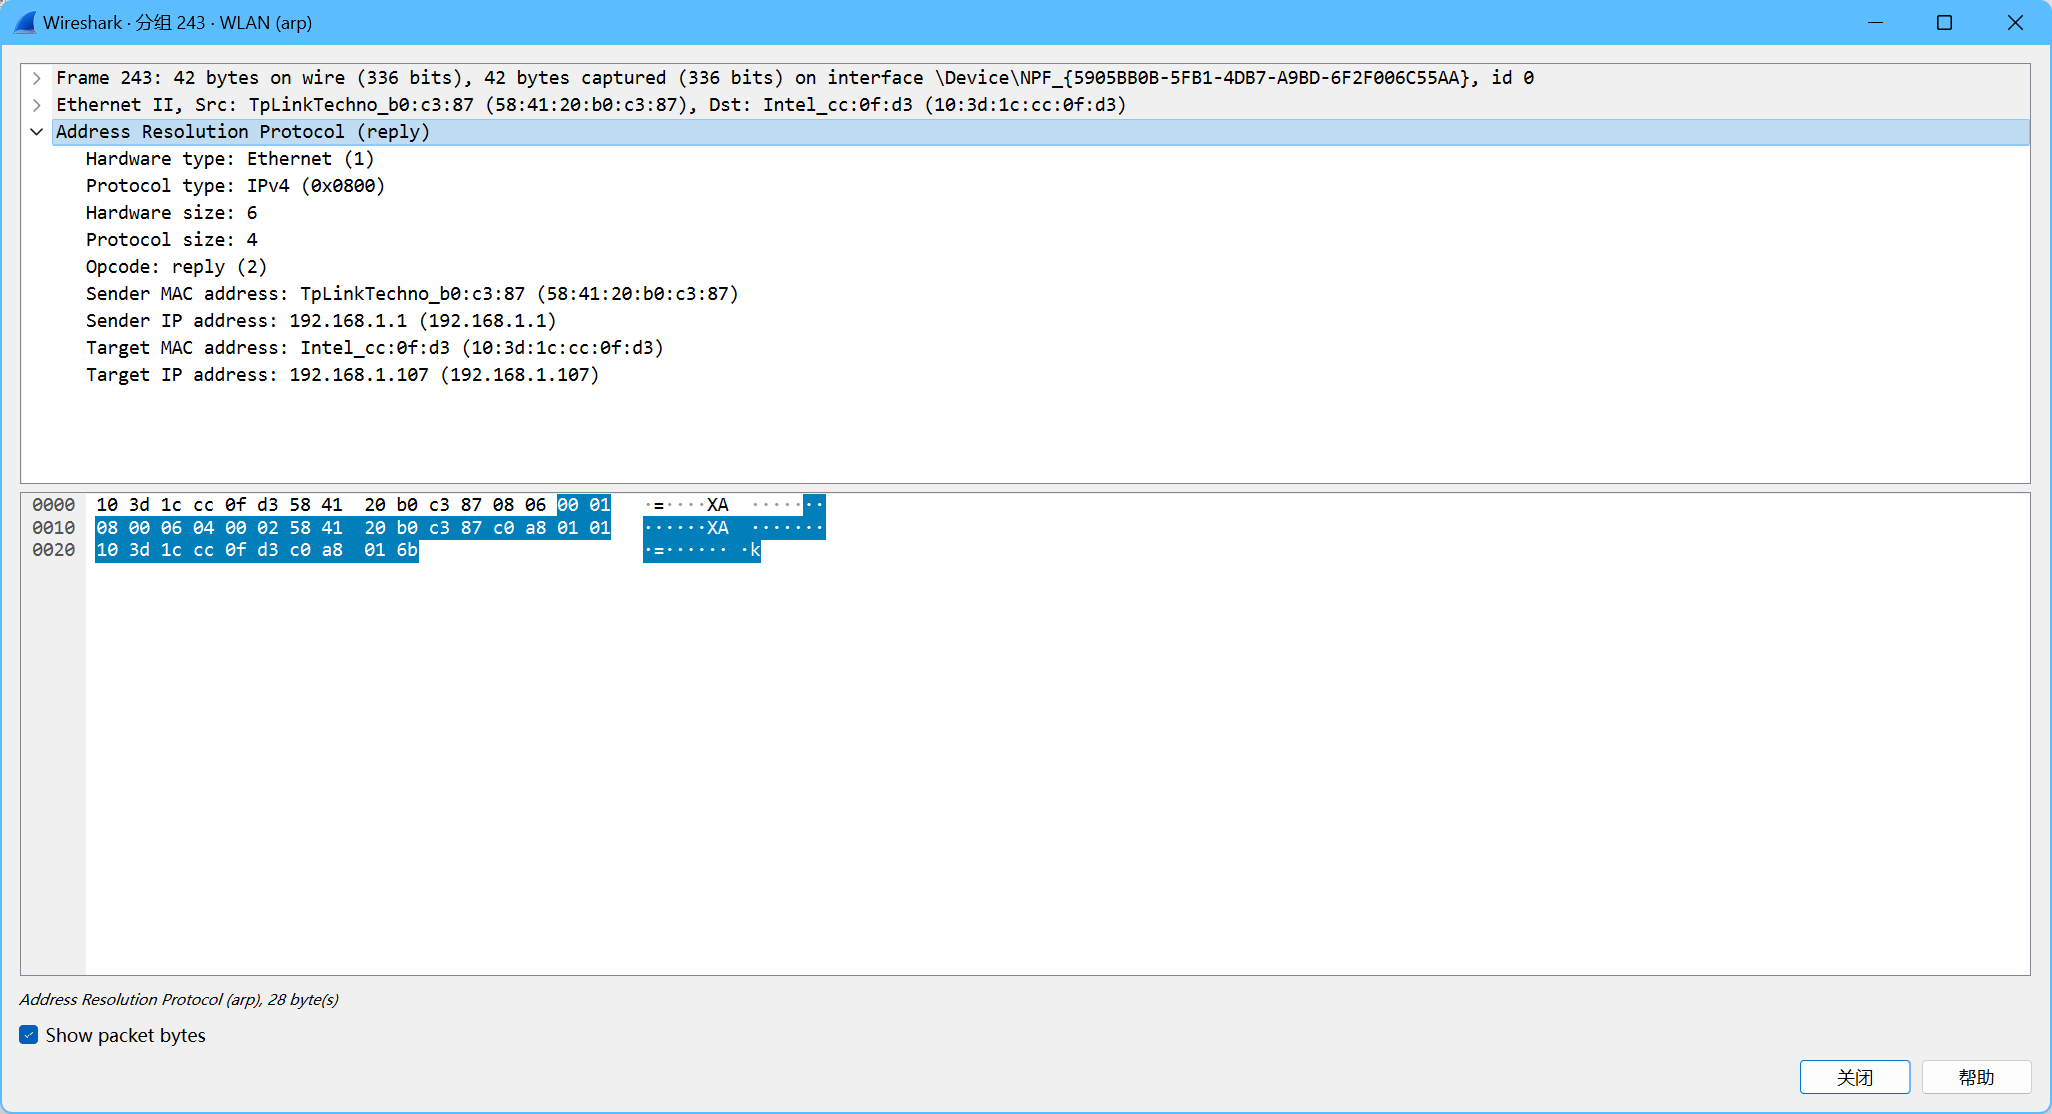
\includegraphics[width=0.8\textwidth]{img/7.png}
          \caption{选择\texttt{ARP}应答数据包}
          \label{fig:7}
        \end{figure}

        画出 \texttt{ARP} 应答数据包,如下图所示:

        % 10 列的表格
        \begin{table}[H]
          \centering
          \begin{tabularx}{0.78\textwidth}{|*{10}{X|}}
            \hline
            \multicolumn{2}{|c|}{Hardware type}      & \multicolumn{2}{c|}{Protocol type}     & \multicolumn{1}{c|}{Hardware size} & \multicolumn{1}{c|}{Protocol size} & \multicolumn{2}{c|}{Opcode} & \multicolumn{2}{c|}{} \\
            \multicolumn{2}{|c|}{1}                  & \multicolumn{2}{c|}{0x0800}            & \multicolumn{1}{c|}{6}             & \multicolumn{1}{c|}{4}             & \multicolumn{2}{c|}{2}      & \multicolumn{2}{c|}{} \\
            \hline
            \multicolumn{6}{|c|}{Sender MAC address} & \multicolumn{4}{c|}{Sender IP address}                                                                                                                                 \\
            \multicolumn{6}{|c|}{58:41:20:b0:c3:87}  & \multicolumn{4}{c|}{192.168.1.1}                                                                                                                                       \\
            \hline
            \multicolumn{6}{|c|}{Target MAC address} & \multicolumn{4}{c|}{Target IP address}                                                                                                                                 \\
            \multicolumn{6}{|c|}{10:3d:1c:cc:0f:d3}  & \multicolumn{4}{c|}{192.168.1.107}                                                                                                                                     \\
            \hline
          \end{tabularx}
          \caption{\texttt{ARP}应答数据包}
        \end{table}


  \item 什么样的操作码是用来表示一个请求?应答呢?

        \texttt{ARP} 报头中的 \texttt{Opcode} 字段用来表示 \texttt{ARP} 请求或应答,其中 \texttt{Opcode} 为 1 表示请求,为 2 表示应答。

  \item 一个请求的ARP的报头有多大?应答呢?

        长度均为 28 字节。
  \item 对未知目标的MAC地址的请求是什么值?

        对未知目标的 \texttt{MAC} 地址的请求是 \texttt{00:00:00:00:00:00}。
  \item 什么以太网类型值说明ARP是更高一层的协议?

        以太网类型值为 \texttt{0x0806} 说明 \texttt{ARP} 是更高一层的协议。

        \begin{figure}[H]
          \centering
          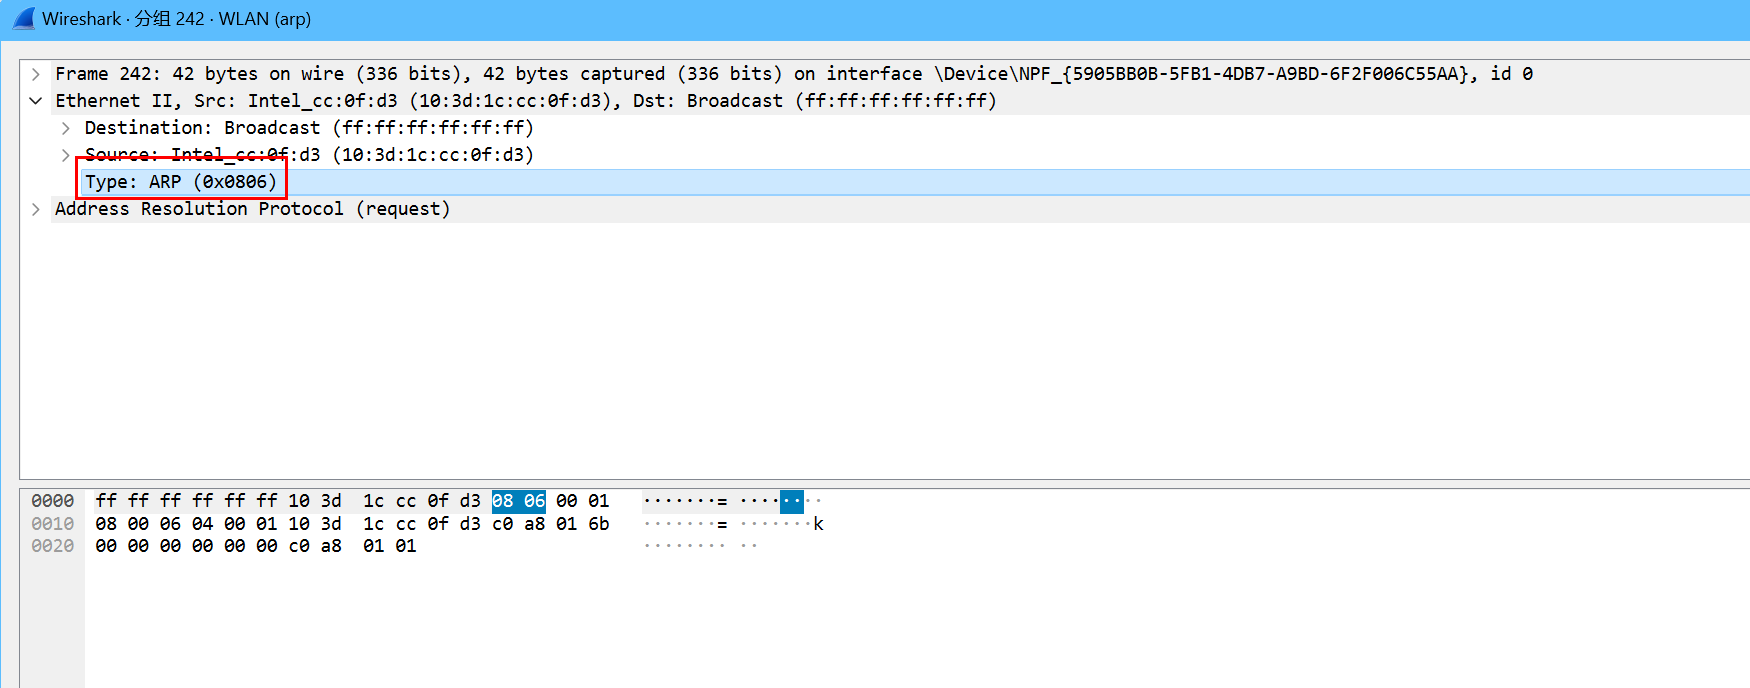
\includegraphics[width=0.8\textwidth]{img/8.png}
          \caption{\texttt{ARP} 的类型值为 \texttt{0x0806}}
          \label{fig:8}
        \end{figure}
  \item ARP应答是广播吗?

        在以太网层可以看出,\texttt{ARP} 应答是单播。

        \begin{figure}[H]
          \centering
          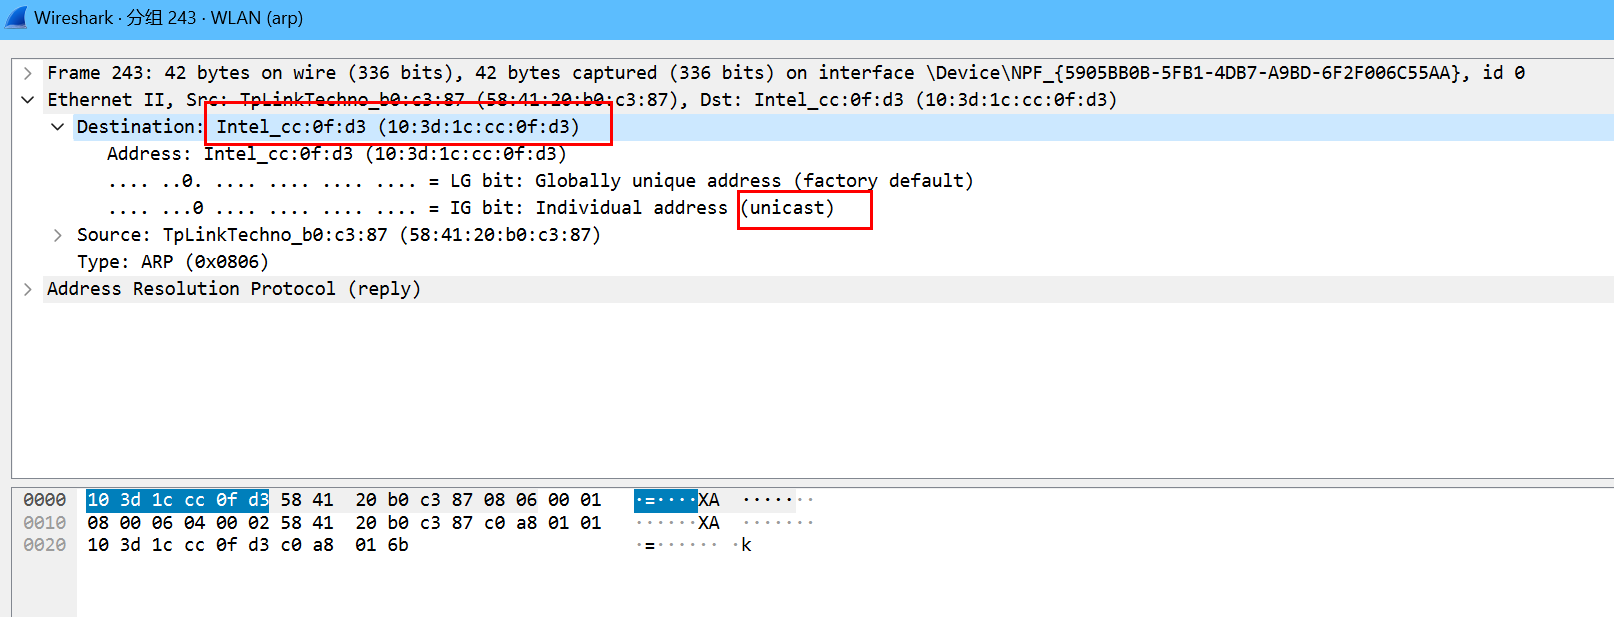
\includegraphics[width=0.8\textwidth]{img/9.png}
          \caption{\texttt{ARP} 应答是单播}
          \label{fig:9}
        \end{figure}

\end{enumerate}

\subsection{问题讨论}

\begin{enumerate}[noitemsep]
\item ARP requests broadcast by other computers. The other computers on the local network are also using ARP. Since requests are broadcast, your computer will receive their requests.

清除筛选后,可以看到其他计算机发送的 \texttt{ARP} 请求。

\begin{figure}[H]
  \centering
  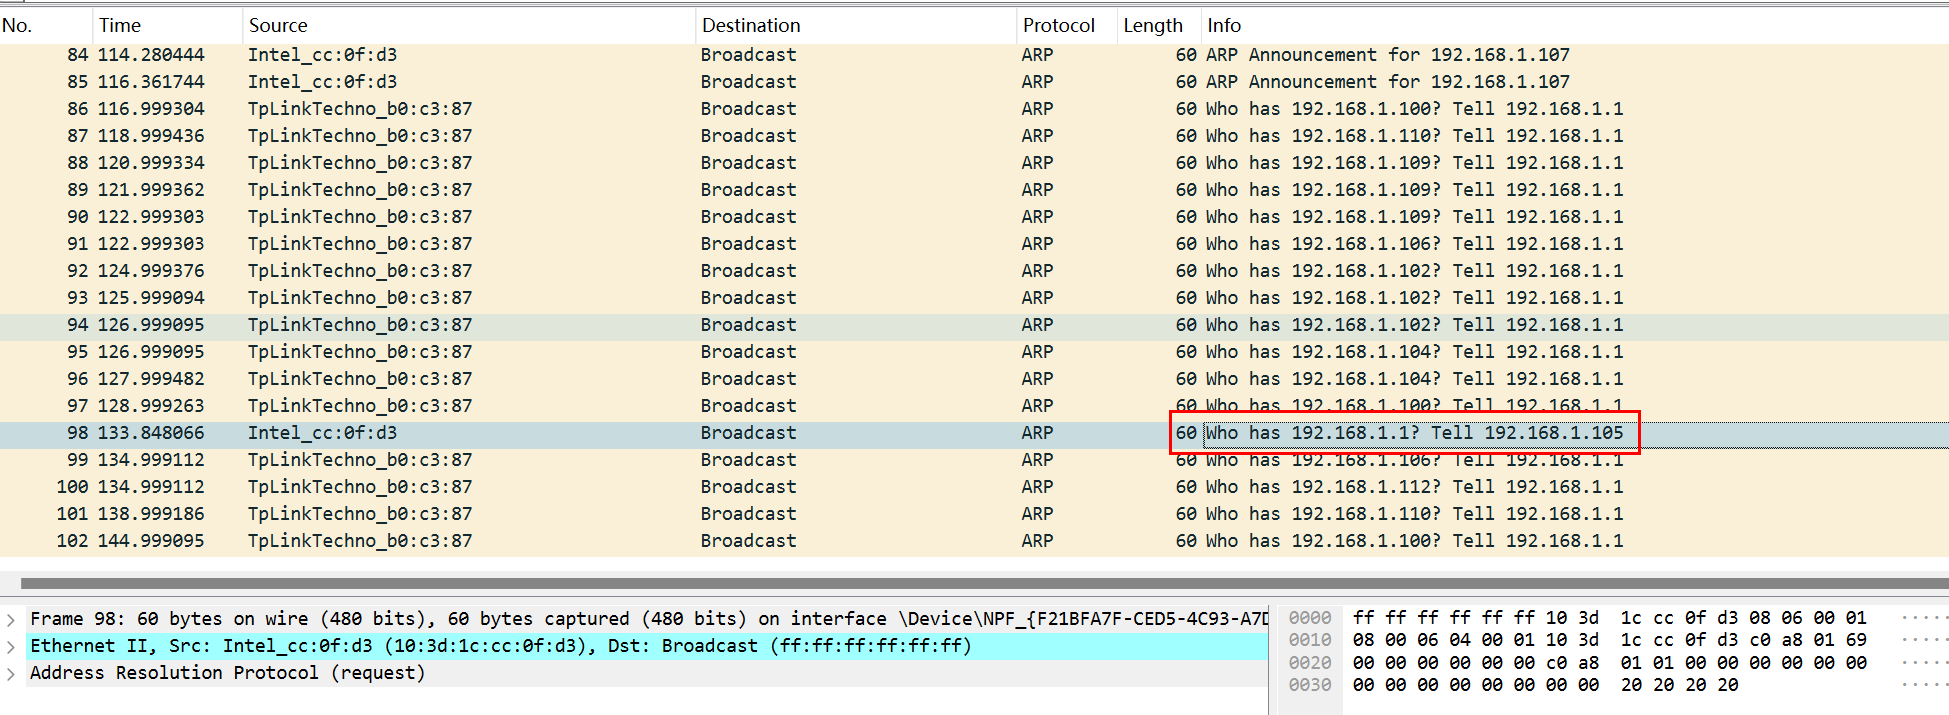
\includegraphics[width=0.8\textwidth]{img/10.png}
  \caption{其他计算机发送的 \texttt{ARP} 请求}
  \label{fig:10}
\end{figure}
\item ARP replies sent by your computer. If another computer happens to ARP for the IP address of your computer, then your computer will send an ARP reply to tell it the answer.

可以在另一台计算机上使用 \texttt{arp -d <Your IP>} 命令清除 \texttt{ARP} 缓存,然后使用 \texttt{ping <Your IP>} 命令向本机发送 \texttt{ICMP} 请求,这时也会发起一个 \texttt{ARP}请求,此时本机会发送 \texttt{ARP} 应答,如下图所示(由于从 \texttt{WIFI} 换到了以太网, \texttt{IP} 地址发生了变化):

\begin{figure}[H]
  \centering
  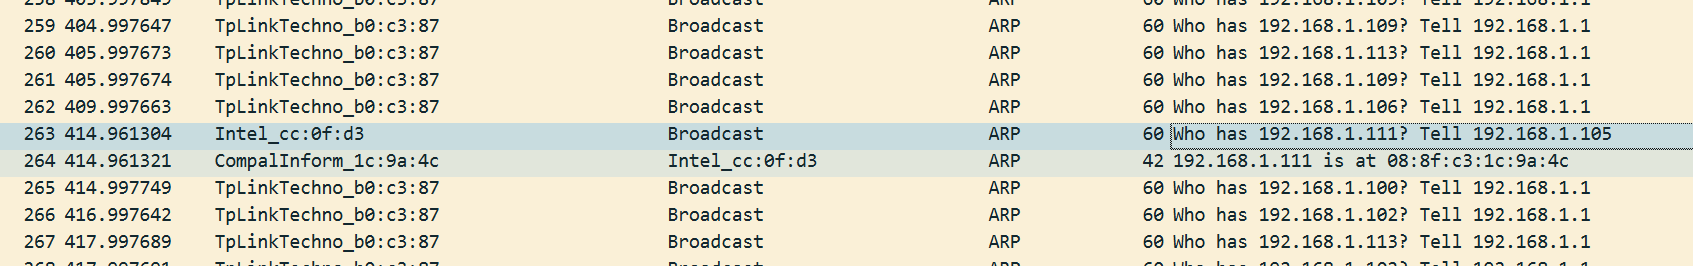
\includegraphics[width=0.8\textwidth]{img/11.png}
  \caption{本机发送了 \texttt{ARP} 应答}
  \label{fig:11}
\end{figure}
\item Gratuitous ARPs in which your computer sends a request or reply about itself. This is helpful when a computer or link comes up to make sure that no-one else is using the same IP address. Gratuitous ARPs have the same sender and target IP address, and they have an Info field in Wireshark that identified them as gratuitous.

可以在捕获列表中看到 \texttt{gratuitous ARP} 数据包。

\begin{figure}[H]
\centering
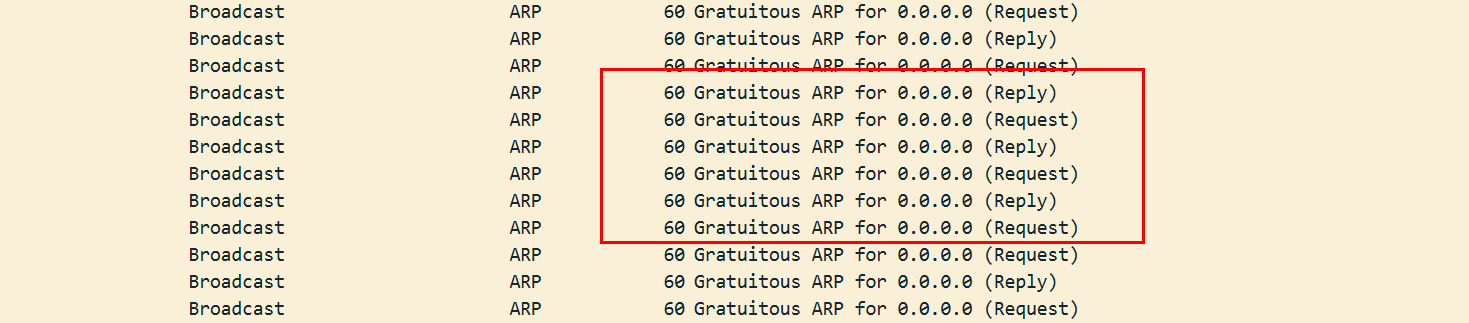
\includegraphics[width=0.8\textwidth]{img/13.png}
\caption{捕获到的 \texttt{gratuitous ARP} 数据包}
\label{fig:13}
\end{figure}
\item Other ARP requests sent by your computer and the corresponding ARP reply. Your computer may need to ARP for other hosts besides the default gateway after you flush its ARP cache.

清除 \texttt{ARP} 缓存后,观察到了相关请求。

\begin{figure}[H]
  \centering
  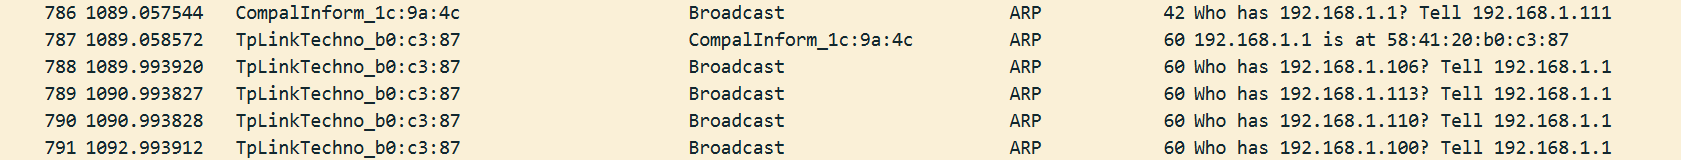
\includegraphics[width=0.8\textwidth]{img/12.png}
  \caption{相关请求}
  \label{fig:12}
\end{figure}

\end{enumerate}


\section{实验结果总结}

本次实验通过 \texttt{Wireshark} 捕获了 \texttt{ARP} 数据包,并对其进行了分析,了解了 \texttt{ARP} 数据包的结构和各字段的含义,进一步增强了对 \texttt{ARP} 协议的理解。


\section{附录}

无

\end{document}